\chapter{Evaluation}
\label{cha:eval}


2/3 packet loss without delay!!! 1 core to 1 core
for large numbers (10,000) packet loss increases to 3/4. Packets above that result in WDOG state at the receiver end.
maybe more reliability with a layer on top of UDP, which would be more expensive/slow


Comparison with two of the most popular RAM-based Key-value pair databases: \textbf{memcached} and \textbf{Redis}.
Run on an ASUS X555L quadcore Intel(R) Core(TM) i5-5200U CPU @ 2.20GHz, 8gb DDR3 RAM @ 1600 MHz.

Write speed with different data sizes, etc.

256 is the limit data size of sdp messages...

As can be seen in figure XXX, the SpiNNaker Database (SpiDB) on the 4 chip board performs quite poorly against the two, running at around 7k put operations per second, compared to ... (thus slow by a factor of about 8) 

complexity


\begin{figure}
\begin{center}
	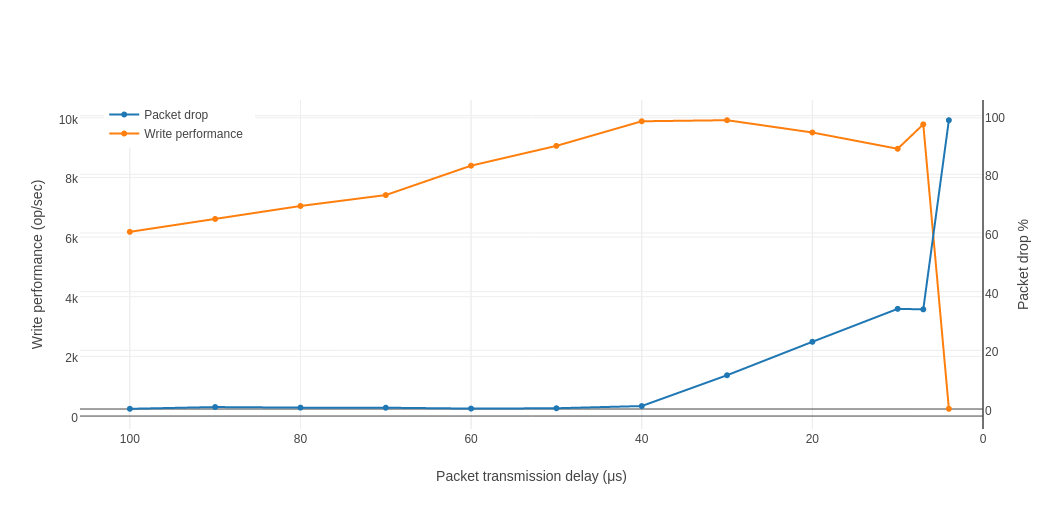
\includegraphics[width=1.4\textwidth, natwidth=1063, natheight=509]{images/transmission_delay.png}
\end{center}
\caption{Transmission delay plot}
\label{fig:transmission-delay}
\end{figure}

%\caption{Die plot of the SpiNNaker CMP}


\lstinputlisting[language=C, caption=SDP Packet Callback]{code/sdp_packet_callback.c}

callback priorities etc.

cannot possibly do more than that...
ARM968 at only 600MHz (I think)

response times. why are they so high sometimes?!?!
-first explain how we gather the time (operating system could be interrupting, sark, etc.)


hash vs naive


HOW ABOUT ALL SEQUENTIAL (dots) VS ALL PARALLEL????



\section{Limitations}

\section{Predictions}

\section{Future work}
future work...
cache (on DTCM)
aggregation
CGI server
self balancing when IDLE (ie. move data to cores with less data, if a table is about to get full, move data around it's SDRAM) --- user typing = a long time
million core machine
improve parser
allow longer queries in (more than 256 bytes)
additional operations eg. delete, update, etc,...
more reliability
ACID properties